\documentclass[a4paper,12pt,oneside]{book}
\usepackage[italian]{babel}
\usepackage[utf8]{inputenc}
\usepackage{textcomp}
\usepackage[parfill]{parskip} %Se necessatrio non indenta, ma inserisce spazio
\usepackage{graphicx}
\usepackage{hyperref}
\usepackage{amsmath} %To number equations

\usepackage{titling}
\newcommand{\subtitle}[1]{%
 \posttitle{%
 \par\end{center}
 \begin{center}\large#1\end{center}
 \vskip6.5em}%
}

\author{Andrea Onofri e Dario Sacco}
\date{Update: v. 1.0 (15/03/2021), compil. 2021-04-28}
\title{Metodologia sperimentale per le scienze agrarie}
\subtitle{}


%***************************************************************

%Specific RMarkdown
\usepackage{color}
\usepackage{fancyvrb}
\usepackage{longtable}
\usepackage{booktabs}
\providecommand{\tightlist}{%
  \setlength{\itemsep}{0pt}\setlength{\parskip}{0pt}}
\newcommand{\VerbBar}{|}
\newcommand{\VERB}{\Verb[commandchars=\\\{\}]}
\DefineVerbatimEnvironment{Highlighting}{Verbatim}{commandchars=\\\{\},fontsize=\small}
\usepackage{framed}
%\newenvironment{Shaded}{}{}
\newenvironment{Shaded}{\begin{snugshade}}{\end{snugshade}}
\definecolor{shadecolor}{RGB}{250,248,248}
\newcommand{\KeywordTok}[1]{#1}
\newcommand{\DataTypeTok}[1]{#1}
\newcommand{\DecValTok}[1]{#1}
\newcommand{\BaseNTok}[1]{#1}
\newcommand{\FloatTok}[1]{#1}
\newcommand{\ConstantTok}[1]{#1}
\newcommand{\CharTok}[1]{#1}
\newcommand{\SpecialCharTok}[1]{#1}
\newcommand{\StringTok}[1]{#1}
\newcommand{\VerbatimStringTok}[1]{#1}
\newcommand{\SpecialStringTok}[1]{#1}
\newcommand{\ImportTok}[1]{#1}
\newcommand{\CommentTok}[1]{#1}
\newcommand{\DocumentationTok}[1]{#1}
\newcommand{\AnnotationTok}[1]{#1}
\newcommand{\CommentVarTok}[1]{#1}
\newcommand{\OtherTok}[1]{#1}
\newcommand{\FunctionTok}[1]{#1}
\newcommand{\VariableTok}[1]{#1}
\newcommand{\ControlFlowTok}[1]{#1}
\newcommand{\OperatorTok}[1]{#1}
\newcommand{\BuiltInTok}[1]{#1}
\newcommand{\ExtensionTok}[1]{#1}
\newcommand{\PreprocessorTok}[1]{#1}
\newcommand{\AttributeTok}[1]{#1}
\newcommand{\RegionMarkerTok}[1]{#1}
\newcommand{\InformationTok}[1]{#1}
\newcommand{\WarningTok}[1]{#1}
\newcommand{\AlertTok}[1]{#1}
\newcommand{\ErrorTok}[1]{#1}
\newcommand{\NormalTok}[1]{#1}
% Redefine \includegraphics so that, unless explicit options are
% given, the image width will not exceed the width of the page.
% Images get their normal width if they fit onto the page, but
% are scaled down if they would overflow the margins.

\begin{document}

\maketitle
\tableofcontents

\hypertarget{premessa}{%
\chapter*{Premessa}\label{premessa}}
\addcontentsline{toc}{chapter}{Premessa}

Placeholder

\hypertarget{obiettivi}{%
\section*{Obiettivi}\label{obiettivi}}
\addcontentsline{toc}{section}{Obiettivi}

\hypertarget{organizzazione}{%
\section*{Organizzazione}\label{organizzazione}}
\addcontentsline{toc}{section}{Organizzazione}

\hypertarget{software-statistico}{%
\section*{Software statistico}\label{software-statistico}}
\addcontentsline{toc}{section}{Software statistico}

\hypertarget{the-authors}{%
\section*{The authors}\label{the-authors}}
\addcontentsline{toc}{section}{The authors}

\hypertarget{ringraziamenti}{%
\section*{Ringraziamenti}\label{ringraziamenti}}
\addcontentsline{toc}{section}{Ringraziamenti}

\hypertarget{scienza-e-pseudo-scienza}{%
\chapter{Scienza e pseudo-scienza}\label{scienza-e-pseudo-scienza}}

Placeholder

\hypertarget{scienza-dati}{%
\section{Scienza = dati}\label{scienza-dati}}

\hypertarget{dati-buoni-e-cattivi}{%
\section{Dati `buoni' e `cattivi'}\label{dati-buoni-e-cattivi}}

\hypertarget{dati-buoni-e-metodi-buoni}{%
\section{Dati `buoni' e metodi `buoni'}\label{dati-buoni-e-metodi-buoni}}

\hypertarget{il-principio-di-falsificazione}{%
\section{Il principio di falsificazione}\label{il-principio-di-falsificazione}}

\hypertarget{falsificare-un-risultato}{%
\section{Falsificare un risultato}\label{falsificare-un-risultato}}

\hypertarget{elementi-fondamentali-del-disegno-sperimentale}{%
\section{Elementi fondamentali del disegno sperimentale}\label{elementi-fondamentali-del-disegno-sperimentale}}

\hypertarget{controllo-degli-errori}{%
\subsection{Controllo degli errori}\label{controllo-degli-errori}}

\hypertarget{replicazione}{%
\subsection{Replicazione}\label{replicazione}}

\hypertarget{randomizzazione}{%
\subsection{Randomizzazione}\label{randomizzazione}}

\hypertarget{esperimenti-invalidi}{%
\subsection{Esperimenti invalidi}\label{esperimenti-invalidi}}

\hypertarget{cattivo-controllo-degli-errori}{%
\subsubsection{Cattivo controllo degli errori}\label{cattivo-controllo-degli-errori}}

\hypertarget{confounding-e-correlazione-spuria}{%
\subsubsection{`Confounding' e correlazione spuria}\label{confounding-e-correlazione-spuria}}

\hypertarget{pseudo-repliche-e-randomizzazione-poco-attenta}{%
\subsubsection{Pseudo-repliche e randomizzazione poco attenta}\label{pseudo-repliche-e-randomizzazione-poco-attenta}}

\hypertarget{chi-valuta-se-un-esperimento-uxe8-attendibile}{%
\section{Chi valuta se un esperimento è attendibile?}\label{chi-valuta-se-un-esperimento-uxe8-attendibile}}

\hypertarget{conclusioni}{%
\section{Conclusioni}\label{conclusioni}}

\hypertarget{altre-letture}{%
\section{Altre letture}\label{altre-letture}}

\hypertarget{progettare-un-esperimento}{%
\chapter{Progettare un esperimento}\label{progettare-un-esperimento}}

Placeholder

\hypertarget{gli-elementi-della-ricerca}{%
\section{Gli elementi della ricerca}\label{gli-elementi-della-ricerca}}

\hypertarget{ipotesi-scientifica-rightarrow-obiettivo-dellesperimento}{%
\section{\texorpdfstring{Ipotesi scientifica \(\rightarrow\) obiettivo dell'esperimento}{Ipotesi scientifica \textbackslash rightarrow obiettivo dell'esperimento}}\label{ipotesi-scientifica-rightarrow-obiettivo-dellesperimento}}

\hypertarget{identificazione-dei-fattori-sperimentali}{%
\section{Identificazione dei fattori sperimentali}\label{identificazione-dei-fattori-sperimentali}}

\hypertarget{esperimenti-multi-fattoriali}{%
\subsection{Esperimenti (multi-)fattoriali}\label{esperimenti-multi-fattoriali}}

\hypertarget{controllo-o-testimone}{%
\subsection{Controllo o testimone}\label{controllo-o-testimone}}

\hypertarget{le-unituxe0-sperimentali}{%
\section{Le unità sperimentali}\label{le-unituxe0-sperimentali}}

\hypertarget{allocazione-dei-trattamenti}{%
\section{Allocazione dei trattamenti}\label{allocazione-dei-trattamenti}}

\hypertarget{le-variabili-sperimentali}{%
\section{Le variabili sperimentali}\label{le-variabili-sperimentali}}

\hypertarget{variabili-nominali-categoriche}{%
\subsection{Variabili nominali (categoriche)}\label{variabili-nominali-categoriche}}

\hypertarget{variabili-ordinali}{%
\subsection{Variabili ordinali}\label{variabili-ordinali}}

\hypertarget{variabili-quantitative-discrete}{%
\subsection{Variabili quantitative discrete}\label{variabili-quantitative-discrete}}

\hypertarget{variabili-quantitative-continue}{%
\subsection{Variabili quantitative continue}\label{variabili-quantitative-continue}}

\hypertarget{rilievi-visivi-e-sensoriali}{%
\subsection{Rilievi visivi e sensoriali}\label{rilievi-visivi-e-sensoriali}}

\hypertarget{variabili-di-confondimento}{%
\subsection{Variabili di confondimento}\label{variabili-di-confondimento}}

\hypertarget{esperimenti-di-campo}{%
\section{Esperimenti di campo}\label{esperimenti-di-campo}}

\hypertarget{scegliere-il-campo}{%
\subsection{Scegliere il campo}\label{scegliere-il-campo}}

\hypertarget{le-unituxe0-sperimentali-in-campo}{%
\subsection{Le unità sperimentali in campo}\label{le-unituxe0-sperimentali-in-campo}}

\hypertarget{numero-di-repliche}{%
\subsection{Numero di repliche}\label{numero-di-repliche}}

\hypertarget{la-mappa-di-campo}{%
\subsection{La mappa di campo}\label{la-mappa-di-campo}}

\hypertarget{lay-out-sperimentale}{%
\subsection{Lay-out sperimentale}\label{lay-out-sperimentale}}

\hypertarget{disegni-completamente-randomizzati}{%
\subsubsection{Disegni completamente randomizzati}\label{disegni-completamente-randomizzati}}

\hypertarget{disegni-a-blocchi-randomizzati}{%
\subsubsection{Disegni a blocchi randomizzati}\label{disegni-a-blocchi-randomizzati}}

\hypertarget{disegni-a-quadrato-latino}{%
\subsubsection{Disegni a quadrato latino}\label{disegni-a-quadrato-latino}}

\hypertarget{disegni-a-split-plot}{%
\subsubsection{Disegni a split-plot}\label{disegni-a-split-plot}}

\hypertarget{disegni-a-strip-plot}{%
\subsubsection{Disegni a strip-plot}\label{disegni-a-strip-plot}}

\hypertarget{altre-letture-1}{%
\section{Altre letture}\label{altre-letture-1}}

\hypertarget{richiami-di-statistica-descrittiva}{%
\chapter{Richiami di statistica descrittiva}\label{richiami-di-statistica-descrittiva}}

Placeholder

\hypertarget{dati-quantitativi}{%
\section{Dati quantitativi}\label{dati-quantitativi}}

\hypertarget{indicatori-di-tendenza-centrale}{%
\subsection{Indicatori di tendenza centrale}\label{indicatori-di-tendenza-centrale}}

\hypertarget{indicatori-di-dispersione}{%
\subsection{Indicatori di dispersione}\label{indicatori-di-dispersione}}

\hypertarget{incertezza-delle-misure-derivate}{%
\subsection{Incertezza delle misure derivate}\label{incertezza-delle-misure-derivate}}

\hypertarget{relazioni-tra-variabili-quantitative-correlazione}{%
\subsection{Relazioni tra variabili quantitative: correlazione}\label{relazioni-tra-variabili-quantitative-correlazione}}

\hypertarget{dati-qualitativi}{%
\section{Dati qualitativi}\label{dati-qualitativi}}

\hypertarget{distribuzioni-di-frequenze-e-classamento}{%
\subsection{Distribuzioni di frequenze e classamento}\label{distribuzioni-di-frequenze-e-classamento}}

\hypertarget{statistiche-descrittive-per-le-distribuzioni-di-frequenze}{%
\subsection{Statistiche descrittive per le distribuzioni di frequenze}\label{statistiche-descrittive-per-le-distribuzioni-di-frequenze}}

\hypertarget{distribuzioni-di-frequenza-bivariate-le-tabelle-di-contingenze}{%
\subsection{Distribuzioni di frequenza bivariate: le tabelle di contingenze}\label{distribuzioni-di-frequenza-bivariate-le-tabelle-di-contingenze}}

\hypertarget{connessione}{%
\subsection{Connessione}\label{connessione}}

\hypertarget{statistiche-descrittive-con-r}{%
\section{Statistiche descrittive con R}\label{statistiche-descrittive-con-r}}

\hypertarget{descrizione-dei-sottogruppi}{%
\subsection{Descrizione dei sottogruppi}\label{descrizione-dei-sottogruppi}}

\hypertarget{distribuzioni-di-frequenze-e-classamento-1}{%
\subsection{Distribuzioni di frequenze e classamento}\label{distribuzioni-di-frequenze-e-classamento-1}}

\hypertarget{connessione-1}{%
\subsection{Connessione}\label{connessione-1}}

\hypertarget{altre-letture-2}{%
\section{Altre letture}\label{altre-letture-2}}

\hypertarget{modelli-statistici-ed-analisi-dei-dati}{%
\chapter{Modelli statistici ed analisi dei dati}\label{modelli-statistici-ed-analisi-dei-dati}}

Placeholder

\hypertarget{verituxe0-vera-e-modelli-deterministici}{%
\section{Verità `vera' e modelli deterministici}\label{verituxe0-vera-e-modelli-deterministici}}

\hypertarget{genesi-deterministica-delle-osservazioni-sperimentali}{%
\section{Genesi deterministica delle osservazioni sperimentali}\label{genesi-deterministica-delle-osservazioni-sperimentali}}

\hypertarget{errore-sperimentale-e-modelli-stocastici}{%
\section{Errore sperimentale e modelli stocastici}\label{errore-sperimentale-e-modelli-stocastici}}

\hypertarget{funzioni-di-probabilituxe0}{%
\subsection{Funzioni di probabilità}\label{funzioni-di-probabilituxe0}}

\hypertarget{funzioni-di-densituxe0}{%
\subsection{Funzioni di densità}\label{funzioni-di-densituxe0}}

\hypertarget{la-distribuzione-normale-curva-di-gauss}{%
\subsection{La distribuzione normale (curva di Gauss)}\label{la-distribuzione-normale-curva-di-gauss}}

\hypertarget{modelli-a-due-facce}{%
\section{Modelli `a due facce'}\label{modelli-a-due-facce}}

\hypertarget{e-allora}{%
\section{E allora?}\label{e-allora}}

\hypertarget{le-simulazioni-monte-carlo}{%
\section{Le simulazioni Monte Carlo}\label{le-simulazioni-monte-carlo}}

\hypertarget{analisi-dei-dati-e-model-fitting}{%
\section{Analisi dei dati e `model fitting'}\label{analisi-dei-dati-e-model-fitting}}

\hypertarget{modelli-stocastici-non-normali}{%
\section{Modelli stocastici non-normali}\label{modelli-stocastici-non-normali}}

\hypertarget{altre-letture-3}{%
\section{Altre letture}\label{altre-letture-3}}

\hypertarget{stime-ed-incertezza}{%
\chapter{Stime ed incertezza}\label{stime-ed-incertezza}}

Placeholder

\hypertarget{esempio-una-soluzione-erbicida}{%
\section{Esempio: una soluzione erbicida}\label{esempio-una-soluzione-erbicida}}

\hypertarget{analisi-dei-dati-stima-dei-parametri}{%
\subsection{Analisi dei dati: stima dei parametri}\label{analisi-dei-dati-stima-dei-parametri}}

\hypertarget{la-sampling-distribution}{%
\subsection{La `sampling distribution'}\label{la-sampling-distribution}}

\hypertarget{lerrore-standard}{%
\subsection{L'errore standard}\label{lerrore-standard}}

\hypertarget{stima-per-intervallo}{%
\section{Stima per intervallo}\label{stima-per-intervallo}}

\hypertarget{lintervallo-di-confidenza}{%
\section{L'intervallo di confidenza}\label{lintervallo-di-confidenza}}

\hypertarget{qual-uxe8-il-senso-dellintervallo-di-confidenza}{%
\section{Qual è il senso dell'intervallo di confidenza?}\label{qual-uxe8-il-senso-dellintervallo-di-confidenza}}

\hypertarget{come-presentare-i-risultati-degli-esperimenti}{%
\section{Come presentare i risultati degli esperimenti}\label{come-presentare-i-risultati-degli-esperimenti}}

\hypertarget{alcune-precisazioni}{%
\section{Alcune precisazioni}\label{alcune-precisazioni}}

\hypertarget{campioni-numerosi-e-non}{%
\subsection{Campioni numerosi e non}\label{campioni-numerosi-e-non}}

\hypertarget{popolazioni-gaussiane-e-non}{%
\subsection{Popolazioni gaussiane e non}\label{popolazioni-gaussiane-e-non}}

\hypertarget{analisi-statistica-dei-dati-riassunto-del-percorso-logico}{%
\section{Analisi statistica dei dati: riassunto del percorso logico}\label{analisi-statistica-dei-dati-riassunto-del-percorso-logico}}

\hypertarget{da-ricordare}{%
\section{Da ricordare}\label{da-ricordare}}

\hypertarget{per-approfondire-un-po}{%
\section{Per approfondire un po'\ldots{}}\label{per-approfondire-un-po}}

\hypertarget{coverage-degli-intervalli-di-confidenza}{%
\section{\texorpdfstring{\emph{Coverage} degli intervalli di confidenza}{Coverage degli intervalli di confidenza}}\label{coverage-degli-intervalli-di-confidenza}}

\hypertarget{intervalli-di-confidenza-per-fenomeni-non-normali}{%
\subsection{Intervalli di confidenza per fenomeni non-normali}\label{intervalli-di-confidenza-per-fenomeni-non-normali}}

\hypertarget{altre-letture-4}{%
\section{Altre letture}\label{altre-letture-4}}

\hypertarget{decisioni-ed-incertezza}{%
\chapter{Decisioni ed incertezza}\label{decisioni-ed-incertezza}}

Placeholder

\hypertarget{confronto-tra-due-medie-il-test-t-di-student}{%
\section{Confronto tra due medie: il test t di Student}\label{confronto-tra-due-medie-il-test-t-di-student}}

\hypertarget{lipotesi-nulla-e-alternativa}{%
\subsection{L'ipotesi nulla e alternativa}\label{lipotesi-nulla-e-alternativa}}

\hypertarget{la-statistica-t}{%
\subsection{La statistica T}\label{la-statistica-t}}

\hypertarget{simulazione-monte-carlo}{%
\subsection{Simulazione Monte Carlo}\label{simulazione-monte-carlo}}

\hypertarget{soluzione-formale}{%
\subsection{Soluzione formale}\label{soluzione-formale}}

\hypertarget{interpretazione-del-p-level}{%
\subsection{Interpretazione del P-level}\label{interpretazione-del-p-level}}

\hypertarget{tipologie-alternative-di-test-t-di-student}{%
\subsection{Tipologie alternative di test t di Student}\label{tipologie-alternative-di-test-t-di-student}}

\hypertarget{confronto-tra-due-proporzioni-il-test-chi2}{%
\section{\texorpdfstring{Confronto tra due proporzioni: il test \(\chi^2\)}{Confronto tra due proporzioni: il test \textbackslash chi\^{}2}}\label{confronto-tra-due-proporzioni-il-test-chi2}}

\hypertarget{simulazione-monte-carlo-1}{%
\subsection{Simulazione Monte Carlo}\label{simulazione-monte-carlo-1}}

\hypertarget{soluzione-formale-1}{%
\subsection{Soluzione formale}\label{soluzione-formale-1}}

\hypertarget{conclusioni-e-riepilogo}{%
\section{Conclusioni e riepilogo}\label{conclusioni-e-riepilogo}}

\hypertarget{altre-letture-5}{%
\section{Altre letture}\label{altre-letture-5}}

\hypertarget{modelli-anova-ad-una-via}{%
\chapter{Modelli ANOVA ad una via}\label{modelli-anova-ad-una-via}}

Placeholder

\hypertarget{caso-studio-confronto-tra-erbicidi-in-vaso}{%
\section{Caso-studio: confronto tra erbicidi in vaso}\label{caso-studio-confronto-tra-erbicidi-in-vaso}}

\hypertarget{descrizione-del-dataset}{%
\section{Descrizione del dataset}\label{descrizione-del-dataset}}

\hypertarget{definizione-di-un-modello-lineare}{%
\section{Definizione di un modello lineare}\label{definizione-di-un-modello-lineare}}

\hypertarget{parametrizzazione-del-modello}{%
\section{Parametrizzazione del modello}\label{parametrizzazione-del-modello}}

\hypertarget{assunzioni-di-base}{%
\section{Assunzioni di base}\label{assunzioni-di-base}}

\hypertarget{fitting-del-modello-metodo-manuale}{%
\section{Fitting del modello: metodo manuale}\label{fitting-del-modello-metodo-manuale}}

\hypertarget{stima-dei-parametri}{%
\subsection{Stima dei parametri}\label{stima-dei-parametri}}

\hypertarget{calcolo-dei-residui}{%
\subsection{Calcolo dei residui}\label{calcolo-dei-residui}}

\hypertarget{stima-di-sigma}{%
\subsection{\texorpdfstring{Stima di \(\sigma\)}{Stima di \textbackslash sigma}}\label{stima-di-sigma}}

\hypertarget{scomposizione-della-varianza}{%
\section{Scomposizione della varianza}\label{scomposizione-della-varianza}}

\hypertarget{test-dipotesi}{%
\section{Test d'ipotesi}\label{test-dipotesi}}

\hypertarget{inferenza-statistica}{%
\section{Inferenza statistica}\label{inferenza-statistica}}

\hypertarget{fitting-del-modello-con-r}{%
\section{Fitting del modello con R}\label{fitting-del-modello-con-r}}

\hypertarget{medie-marginali-attese}{%
\section{Medie marginali attese}\label{medie-marginali-attese}}

\hypertarget{per-concludere}{%
\section{Per concludere \ldots{}}\label{per-concludere}}

\hypertarget{altre-letture-6}{%
\section{Altre letture}\label{altre-letture-6}}

\hypertarget{la-verifica-delle-assunzioni-di-base}{%
\chapter{La verifica delle assunzioni di base}\label{la-verifica-delle-assunzioni-di-base}}

Placeholder

\hypertarget{violazioni-delle-assunzioni-di-base}{%
\section{Violazioni delle assunzioni di base}\label{violazioni-delle-assunzioni-di-base}}

\hypertarget{procedure-diagnostiche}{%
\section{Procedure diagnostiche}\label{procedure-diagnostiche}}

\hypertarget{analisi-grafica-dei-residui}{%
\section{Analisi grafica dei residui}\label{analisi-grafica-dei-residui}}

\hypertarget{grafico-dei-residui-contro-i-valori-attesi}{%
\subsection{Grafico dei residui contro i valori attesi}\label{grafico-dei-residui-contro-i-valori-attesi}}

\hypertarget{qq-plot}{%
\subsection{QQ-plot}\label{qq-plot}}

\hypertarget{test-dipotesi-1}{%
\section{Test d'ipotesi}\label{test-dipotesi-1}}

\hypertarget{risultati-contraddittori}{%
\section{Risultati contraddittori}\label{risultati-contraddittori}}

\hypertarget{terapia}{%
\section{`Terapia'}\label{terapia}}

\hypertarget{correzionerimozione-degli-outliers}{%
\subsection{Correzione/Rimozione degli outliers}\label{correzionerimozione-degli-outliers}}

\hypertarget{correzione-del-modello}{%
\subsection{Correzione del modello}\label{correzione-del-modello}}

\hypertarget{trasformazione-della-variabile-indipendente}{%
\subsection{Trasformazione della variabile indipendente}\label{trasformazione-della-variabile-indipendente}}

\hypertarget{impiego-di-metodiche-statistiche-avanzate}{%
\subsection{Impiego di metodiche statistiche avanzate}\label{impiego-di-metodiche-statistiche-avanzate}}

\hypertarget{trasformazioni-stabilizzanti}{%
\subsection{Trasformazioni stabilizzanti}\label{trasformazioni-stabilizzanti}}

\hypertarget{esempio-1}{%
\section{Esempio 1}\label{esempio-1}}

\hypertarget{esempio-2}{%
\section{Esempio 2}\label{esempio-2}}

\hypertarget{altre-letture-7}{%
\section{Altre letture}\label{altre-letture-7}}

\hypertarget{contrasti-e-confronti-multipli}{%
\chapter{Contrasti e confronti multipli}\label{contrasti-e-confronti-multipli}}

Placeholder

\hypertarget{esempio}{%
\section{Esempio}\label{esempio}}

\hypertarget{i-contrasti}{%
\section{I contrasti}\label{i-contrasti}}

\hypertarget{i-contrasti-con-r}{%
\section{I contrasti con R}\label{i-contrasti-con-r}}

\hypertarget{i-confronti-multipli-a-coppie-pairwise-comparisons}{%
\section{I confronti multipli a coppie (pairwise comparisons)}\label{i-confronti-multipli-a-coppie-pairwise-comparisons}}

\hypertarget{display-a-lettere}{%
\section{Display a lettere}\label{display-a-lettere}}

\hypertarget{tassi-di-errore-per-confronto-e-per-esperimento}{%
\section{Tassi di errore per confronto e per esperimento}\label{tassi-di-errore-per-confronto-e-per-esperimento}}

\hypertarget{aggiustamento-per-la-molteplicituxe0}{%
\section{Aggiustamento per la molteplicità}\label{aggiustamento-per-la-molteplicituxe0}}

\hypertarget{e-le-classiche-procedure-di-confronto-multiplo}{%
\section{E le classiche procedure di confronto multiplo?}\label{e-le-classiche-procedure-di-confronto-multiplo}}

\hypertarget{consigli-pratici}{%
\section{Consigli pratici}\label{consigli-pratici}}

\hypertarget{altre-letture-8}{%
\section{Altre letture}\label{altre-letture-8}}

\hypertarget{modelli-anova-con-fattori-di-blocco}{%
\chapter{Modelli ANOVA con fattori di blocco}\label{modelli-anova-con-fattori-di-blocco}}

Placeholder

\hypertarget{caso-studio-confronto-tra-erbicidi-in-campo}{%
\section{Caso-studio: confronto tra erbicidi in campo}\label{caso-studio-confronto-tra-erbicidi-in-campo}}

\hypertarget{definizione-di-un-modello-lineare-1}{%
\section{Definizione di un modello lineare}\label{definizione-di-un-modello-lineare-1}}

\hypertarget{stima-dei-parametri-1}{%
\section{Stima dei parametri}\label{stima-dei-parametri-1}}

\hypertarget{coefficienti-del-modello}{%
\subsection{Coefficienti del modello}\label{coefficienti-del-modello}}

\hypertarget{stima-di-sigma-1}{%
\subsection{\texorpdfstring{Stima di \(\sigma\)}{Stima di \textbackslash sigma}}\label{stima-di-sigma-1}}

\hypertarget{scomposizione-della-varianza-1}{%
\section{Scomposizione della varianza}\label{scomposizione-della-varianza-1}}

\hypertarget{adattamento-del-modello-con-r}{%
\section{Adattamento del modello con R}\label{adattamento-del-modello-con-r}}

\hypertarget{disegni-a-quadrato-latino-1}{%
\section{Disegni a quadrato latino}\label{disegni-a-quadrato-latino-1}}

\hypertarget{caso-studio-confronto-tra-metodi-costruttivi}{%
\section{Caso studio: confronto tra metodi costruttivi}\label{caso-studio-confronto-tra-metodi-costruttivi}}

\hypertarget{definizione-di-un-modello-lineare-2}{%
\section{Definizione di un modello lineare}\label{definizione-di-un-modello-lineare-2}}

\hypertarget{la-regressione-lineare-semplice}{%
\chapter{La regressione lineare semplice}\label{la-regressione-lineare-semplice}}

Nei capitoli precedenti abbiamo parlato di modelli basati su una fattori sperimentali in forma di categorie, ad esempio diversi erbicidi o diverse varietà. Abbiamo visto che, con questi fattori sperimentali, si utilizzano i cosiddetti modelli ANOVA.

Nella sperimentazione agronomica e, in genere, biologica, la variabile indipendente (o le variabili indipendenti) può (possono) rappresentare una quantità, come, ad esempio, la dose di un farmaco, il tempo trascorso da un certo evento, la fittezza di semina e così via. In questa condizione, l'analisi dei dati richiede modelli diversi da qualli visti finora, di solito identificati con il nome di modelli di regressione. Questa classe di modelli è estremamente interessante e si presta a sviluppi potentissimi. In questo libro ci accontenteremo di trattare la regressione lineare semplice, cioè un modello lineare (retta) con una variabile dipendente ed un regressore. In un capitolo successivo estenderemo le considerazioni fatte ai modelli non-lineari.

\hypertarget{caso-studio-effetto-della-concimazione-azotata-al-frumento}{%
\section{Caso studio: effetto della concimazione azotata al frumento}\label{caso-studio-effetto-della-concimazione-azotata-al-frumento}}

Per individuare la relazione tra la concimazione azotata e la produzione del frumento, è stato organizzato un esperimento a randomizzazione completa, con quattro dosi di azoto e quattro repliche. I risultati ottenuti sono riportati nella Tabella \ref{tab:tabName141} e possono essere caricati direttamente da gitHub, con il codice sottostante. A differenza dei capitoli precedenti, in questo caso il dataset non è ottenuto da una prova vera, ma è stato generato, con il codice riportato nel capitolo 4. Pertanto, l'esempio, pur essendo efficace da un punto di vista didattico, potrebbe non essere assolutamento realistico.

\begin{Shaded}
\begin{Highlighting}[]
\NormalTok{fileName }\OtherTok{\textless{}{-}} \StringTok{"https://www.casaonofri.it/\_datasets/NWheat.csv"}
\NormalTok{dataset }\OtherTok{\textless{}{-}} \FunctionTok{read.csv}\NormalTok{(fileName, }\AttributeTok{header=}\NormalTok{T)}
\end{Highlighting}
\end{Shaded}

\begin{table}

\caption{\label{tab:tabName141}Dataset relativo ad una prova di concimazione azotata su frumento}
\centering
\begin{tabular}[t]{rrrrr}
\toprule{}
Dose & 1 & 2 & 3 & 4\\
\midrule{}
0 & 21.98 & 25.69 & 27.71 & 19.14\\
60 & 35.07 & 35.27 & 32.56 & 32.63\\
120 & 41.59 & 40.77 & 41.81 & 40.50\\
180 & 50.06 & 52.16 & 54.40 & 51.72\\
\bottomrule{}
\end{tabular}
\end{table}

\hypertarget{analisi-preliminari}{%
\section{Analisi preliminari}\label{analisi-preliminari}}

Questo esperimento è replicato ed è totalmente analogo a quello presentato nel capitolo 7, con l'unica differenza che, in questo caso, la variabile indipendente è quantitativa. Tuttavia, è del tutto logico considerare la dose di azoto come un predittore qualitativo (`factor') ed utilizzare un modello descrittivo ANOVA ad una via. Eseguiamo il `fitting' con R, ottenendo i risultati seguenti:

\begin{Shaded}
\begin{Highlighting}[]
\NormalTok{dataset}\SpecialCharTok{$}\NormalTok{DoseF }\OtherTok{\textless{}{-}} \FunctionTok{factor}\NormalTok{(dataset}\SpecialCharTok{$}\NormalTok{Dose)}
\NormalTok{model }\OtherTok{\textless{}{-}} \FunctionTok{lm}\NormalTok{(Yield }\SpecialCharTok{\textasciitilde{}}\NormalTok{ DoseF, }\AttributeTok{data =}\NormalTok{ dataset)}
\FunctionTok{anova}\NormalTok{(model)}
\DocumentationTok{\#\# Analysis of Variance Table}
\DocumentationTok{\#\# }
\DocumentationTok{\#\# Response: Yield}
\DocumentationTok{\#\#           Df  Sum Sq Mean Sq F value    Pr(\textgreater{}F)    }
\DocumentationTok{\#\# DoseF      3 1725.96  575.32  112.77 4.668e{-}09 ***}
\DocumentationTok{\#\# Residuals 12   61.22    5.10                      }
\DocumentationTok{\#\# {-}{-}{-}}
\DocumentationTok{\#\# Signif. codes:  0 \textquotesingle{}***\textquotesingle{} 0.001 \textquotesingle{}**\textquotesingle{} 0.01 \textquotesingle{}*\textquotesingle{} 0.05 \textquotesingle{}.\textquotesingle{} 0.1 \textquotesingle{} \textquotesingle{} 1}
\end{Highlighting}
\end{Shaded}

Osserviamo che l'effetto del trattamento è significativo e il SEM è pari a \(\sqrt{5.10/4} = 1.129\). Prima di proseguire, verifichiamo che non ci siano problemi relativi alle assunzioni parametriche di base e che, quindi, la trasformazione dei dati non sia necessaria. I grafici dei residui, riportati in Figura \ref{fig:figName141}, non mostrano patologie rilevanti.

\begin{figure}

{\centering 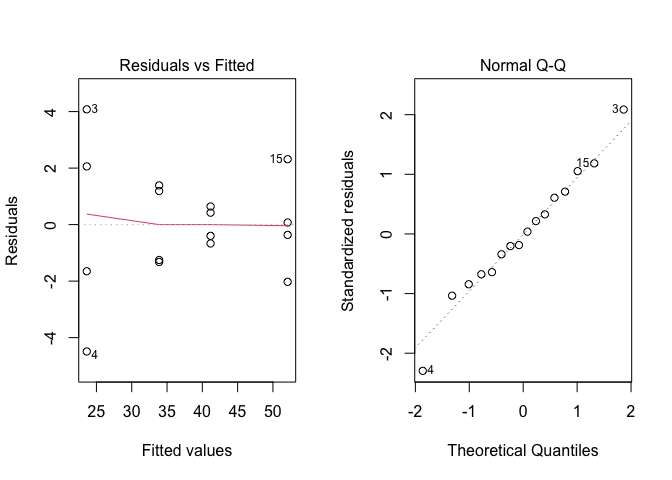
\includegraphics[width=0.9\linewidth]{_main_files/figure-latex/figName141-1} 

}

\caption{Analisi grafica dei residui per una prova di concimazione azotata del frumento}\label{fig:figName141}
\end{figure}

Da questo momento in avanti, diversamente a quanto abbiamo visto nei capitoli precedenti, l'analisi non prosegue con un test di confronto multiplo, che in questa situazione, se non del tutto errato, sarebbe comunque da considerare `improprio.' Infatti, quale senso avrebbe confrontare la risposta produttiva a 60 kg N ha\textsuperscript{-1} con quella a 120 kg N ha \textsuperscript{-1}? In realtà noi non siamo specificatamente interessati a queste due dosi, ma a qualunque altra dose nell'intervallo da 0 a 180 kg N ha\textsuperscript{-1}. Abbiamo selezionato quattro dosi per organizzare l'esperimento, ma resta il fatto che siamo interessati a definire una funzione di risposta per tutto l'intervallo delle dosi, non a confrontare le risposte a due dosi in particolare.

Per questo motivo, quando la variabile indipendente è una dose, l'analisi dei dati dovrebbe essere basata sull'impiego di un modello di regressione, in quanto ciò è più coerente con le finalità dell'esperimento, rispetto all'adozione di una procedura di confronto multiplo.

\hypertarget{definizione-del-modello-lineare}{%
\section{Definizione del modello lineare}\label{definizione-del-modello-lineare}}

Immaginiamo che, almeno nell'intervallo di dosi incluso nell'esperimento, l'effetto della concimazione azotata sulla produzione sia lineare. In effetti, l'andamento dei dati conferma questa impressione e, pertanto, poniamo il modello lineare nei termini usuali:

\[Y_i = b_0 + b_1 X_i + \varepsilon_i\]

dove \(Y\) è la produzione della parcella \(i\), trattata con la dose \(X_i\), \(b_0\) è l'intercetta (produzione a dose di azoto pari a 0) e \(b_1\) è la pendenza, cioè l'incremento di produzione per ogni incremento unitario della dose. La componente stocastica \(\varepsilon\) viene assunta omoscedastica e normalmente distribuita, con media 0 e deviazione standard \(\sigma\).

\hypertarget{stima-dei-parametri-2}{%
\section{Stima dei parametri}\label{stima-dei-parametri-2}}

Dobbiamo a questo punto individuare i parametri \(b_0\) e \(b_1\) in modo tale che la retta ottenuta sia la più vicina ai dati, cioè in modo da minimizzare gli scostamenti tra i valori di produzione osservati e quelli stimati dal modello (soluzione dei minimi quadrati). La funzione dei minimi quadrati è:

\[\begin{array}{l}
Q = \sum\limits_{i = }^N {\left( {{Y_i} - \hat Y} \right)^2 = \sum\limits_{i = }^N {{{\left( {{Y_i} - {b_0} - {b_1}{X_i}} \right)}^2}}  = } \\
 = \sum\limits_{i = }^N {\left( {Y_i^2 + b_0^2 + b_1^2X_i^2 - 2{Y_i}{b_0} - 2{Y_i}{b_1}{X_i} + 2{b_0}{b_1}{X_i}} \right)}  = \\
 = \sum\limits_{i = }^N {Y_i^2 + Nb_0^2 + b_1^2\sum\limits_{i = }^N {X_i^2 - 2{b_0}\sum\limits_{i = }^N {Y_i^2 - 2{b_1}\sum\limits_{i = }^N {{X_i}{Y_i} + } } } } 2{b_0}{b_1}\sum\limits_{i = }^N {{X_i}} 
\end{array}\]

Calcolando le derivate parziali rispetto a \(b_0\) e \(b_1\) che, al momento, sono le nostre incognite, ed eguagliandole a 0 si ottengono le seguenti formule risolutive:

\[{b_1} = \frac{{\sum\limits_{i = 1}^N {\left[ {\left( {{X_i} - {\mu _X}} \right)\left( {{Y_i} - {\mu _Y}} \right)} \right]} }}{{\sum\limits_{i = 1}^N {{{\left( {{X_i} - {\mu _X}} \right)}^2}} }}\]

e:

\[{b_0} = {\mu _Y} - {b_1}{\mu _X}\]

Invece che svolgere i calcoli a mano, possiamo eseguire il fitting ai minimi quadrati con R. Possiamo notare che l'unica differenza tra questo modello di regressione e il modello ANOVA utilizzato poco sopra è che qui utilizziamo la variabile `Dose' come tale, senza prima trasformarla in un `factor.'

\begin{Shaded}
\begin{Highlighting}[]
\NormalTok{modelReg }\OtherTok{\textless{}{-}} \FunctionTok{lm}\NormalTok{(Yield }\SpecialCharTok{\textasciitilde{}}\NormalTok{ Dose, }\AttributeTok{data =}\NormalTok{ dataset)}
\FunctionTok{summary}\NormalTok{(modelReg)}
\DocumentationTok{\#\# }
\DocumentationTok{\#\# Call:}
\DocumentationTok{\#\# lm(formula = Yield \textasciitilde{} Dose, data = dataset)}
\DocumentationTok{\#\# }
\DocumentationTok{\#\# Residuals:}
\DocumentationTok{\#\#     Min      1Q  Median      3Q     Max }
\DocumentationTok{\#\# {-}4.6537 {-}1.5350 {-}0.4637  1.9250  3.9163 }
\DocumentationTok{\#\# }
\DocumentationTok{\#\# Coefficients:}
\DocumentationTok{\#\#              Estimate Std. Error t value Pr(\textgreater{}|t|)    }
\DocumentationTok{\#\# (Intercept) 23.793750   0.937906   25.37 4.19e{-}13 ***}
\DocumentationTok{\#\# Dose         0.154417   0.008356   18.48 3.13e{-}11 ***}
\DocumentationTok{\#\# {-}{-}{-}}
\DocumentationTok{\#\# Signif. codes:  0 \textquotesingle{}***\textquotesingle{} 0.001 \textquotesingle{}**\textquotesingle{} 0.01 \textquotesingle{}*\textquotesingle{} 0.05 \textquotesingle{}.\textquotesingle{} 0.1 \textquotesingle{} \textquotesingle{} 1}
\DocumentationTok{\#\# }
\DocumentationTok{\#\# Residual standard error: 2.242 on 14 degrees of freedom}
\DocumentationTok{\#\# Multiple R{-}squared:  0.9606, Adjusted R{-}squared:  0.9578 }
\DocumentationTok{\#\# F{-}statistic: 341.5 on 1 and 14 DF,  p{-}value: 3.129e{-}11}
\end{Highlighting}
\end{Shaded}

Ora sappiamo che la relazione tra la dose di azoto e la risposta produttiva del frumento è:

\[ Y_i = 23.111 + 0.1544 \times X_i \]

L'elemento stocastico \(\varepsilon_i\) è normalmente distribuito, con media 0 e deviazione standard 2.029 (vedi la voce `Residual standard error' nell'output sovrstante).

Come al solito, prima di qualunque altra considerazione, dobbiamo verificare la bontà del modello e il rispetto delle assunzioni di base, con una procedura che, per un modello di regressione, deve riguardare un maggior numero di aspetti rispetto ad un modello ANOVA.

\hypertarget{valutazione-della-bontuxe0-del-modello}{%
\section{Valutazione della bontà del modello}\label{valutazione-della-bontuxe0-del-modello}}

In primo luogo, è necessario verificare il rispetto delle assunzioni di base di normalità e omoscedasticità dei residui. Per questo, possiamo utilizzare gli stessi metodi impiegati per i modelli ANOVA, vale a dire un grafico dei residui verso gli attesi ed un QQ-plot dei residui standardizzati. In realtà, abbiamo già eseguito questo controllo con il modello ANOVA corrispondente e non vi è la necessità di ripeterlo con questo modello.

Dobbiamo invece assicurarci che i dati osservati siano ben descritti dal modello adottato, senza nessuna componente sistematica di mancanza d'adattamento. In altre parole, le osservazioni non debbono contraddire l'ipotesi che la risposta è lineare, salvo per le eventuali deviazioni casuali insite in qualunque esperimento. Per la verificà della \textbf{bontà di adattamento} possiamo utilizzare diverse procedure, che illustreremo di seguito.

\hypertarget{valutazione-grafica}{%
\subsection{Valutazione grafica}\label{valutazione-grafica}}

Nel modo più semplice, la bontà di adattamento può essere valutata attraverso un grafico dei valori attesi e dei valori osservati, come quello in Figura \ref{fig:figName142}. Notiamo che non c'è alcun elemento che faccia pensare ad una sistematica deviazione rispetto alle previsioni fatte dal modello.

\begin{figure}

{\centering 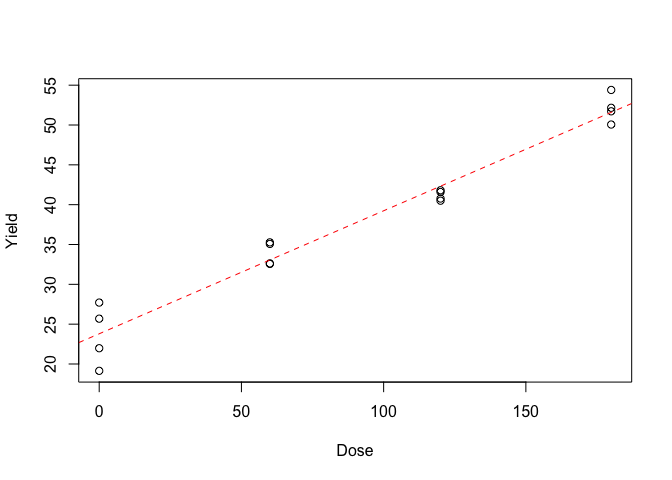
\includegraphics[width=0.9\linewidth]{_main_files/figure-latex/figName142-1} 

}

\caption{Risposta produttiva del frumento alla concimazione azotata: dati osservati (simboli) e valori attesi (linea tratteggiata).}\label{fig:figName142}
\end{figure}

\hypertarget{errori-standard-dei-parametri}{%
\subsection{Errori standard dei parametri}\label{errori-standard-dei-parametri}}

In secondo luogo, possiamo valutare gli errori standard delle stime dei parametri, che non debbono mai essere superiori alla metà del valore del parametro stimato, cosa che in questo caso è pienamente verificata. Se così non fosse, l'intervallo di confidenza del parametro, usualmente stimato utilizzando il doppio dell'errore standard, conterrebbe lo zero, il che equivarebbe a dire che, ad esempio, la pendenza `vera' (cioè quella della popolazione da cui il nostro campione è estratto) potrebbe essere nulla. In altre parole, la retta potrebbe essere `piatta,' dimostrando l'inesistenza di relazione tra la dose di concimazione e la produzione della coltura. Si può notare che, nell'esempio in studio, questo dubbio non sembra sussistere.

\hypertarget{test-f-per-la-mancanza-dadattamento}{%
\subsection{Test F per la mancanza d'adattamento}\label{test-f-per-la-mancanza-dadattamento}}

In terzo luogo, possiamo analizzare i residui della regressione, cioè gli scostamenti dei punti rispetto alla retta e, in particolare, la somma dei loro quadrati. Possiamo vedere che questo valore è pari a 70.37, ed è più alto di quello del corrispondente modello ANOVA, impiegato in precedenza (61.22):

\begin{Shaded}
\begin{Highlighting}[]
\FunctionTok{anova}\NormalTok{(modelReg)}
\DocumentationTok{\#\# Analysis of Variance Table}
\DocumentationTok{\#\# }
\DocumentationTok{\#\# Response: Yield}
\DocumentationTok{\#\#           Df  Sum Sq Mean Sq F value    Pr(\textgreater{}F)    }
\DocumentationTok{\#\# Dose       1 1716.80 1716.80  341.54 3.129e{-}11 ***}
\DocumentationTok{\#\# Residuals 14   70.37    5.03                      }
\DocumentationTok{\#\# {-}{-}{-}}
\DocumentationTok{\#\# Signif. codes:  0 \textquotesingle{}***\textquotesingle{} 0.001 \textquotesingle{}**\textquotesingle{} 0.01 \textquotesingle{}*\textquotesingle{} 0.05 \textquotesingle{}.\textquotesingle{} 0.1 \textquotesingle{} \textquotesingle{} 1}
\end{Highlighting}
\end{Shaded}

Il risultato è perfettamente normale, dato che il residuo del modello ANOVA contiene solo la misura dello scostamento di ogni dato rispetto alla media del suo gruppo, che si può considerare `errore puro,' mentre il residuo della regressione, oltre all'errore puro, contiene anche una componente detta `mancanza d'adattamento' (\emph{lack of fit}), misurabile con lo scostamento di ogni media dalla linea di regressione. In effetti, la regressione lineare è solo un'approssimazione della reale relazione biologica tra la concimazione e la produzione del frumento.

Insomma, il modello di regressione è un modello che ha sempre minor capacità descrittiva rispetto ad un modello ANOVA. La differenza può essere quantificata utilizzando le devianze dei rispettivi residui:

\[\textrm{Lack of fit} = 70.37 - 61.22 = 9.15\]

Bisogna però anche dire che il modello di regressione è più parsimonioso, nel senso che ci ha costretto a stimare solo due parametri (\(b_0\) e \(b_1\)), mentre il modello ANOVA ce ne ha fatti stimare quattro (\(\mu\), \(\alpha_2\), \(\alpha_3\) e \(\alpha_4\), considerando che \(\alpha_1 = 0\)). Quindi il residuo del modello di regressione ha 14 gradi di libertà (16 dati meno due parametri stimati), mentre il residuo del modello ANOVA ne ha 12 (16 - 4). La componente di lack of fit ha quindi 14 - 12 = 2 gradi di libertà. Ci chiediamo, questa componente di lack of fit è significativamente più grande dell'errore puro?

L'ipotesi nulla di assenza di lack of fit può essere testata con un test di F, per il confronto di due varianze: se questo è significativo allora la componente di mancanza d'adattamento non è trascurabile, ed il modello di regressione dovrebbe essere rifiutato. L'espressione è:

\[ F_{lack} = \frac{\frac{RSS_r - RSS_a}{DF_r-DF_a} } {\frac{RSS_a}{DF_a}} = \frac{MS_{lack}}{MSE_a}\]

dove RSS\textsubscript{r} è la devianza residua della regressione con i sui gradi di liberta DF\textsubscript{r} e RSS\textsubscript{a} è la devianza residua del modello ANOVA, con i suoi gradi di libertà DF\textsubscript{a}. In R, il test F per la mancanza d'adattamento può essere eseguito con la funzione \texttt{anova()}, confrontando i due modelli alternativi:

\begin{Shaded}
\begin{Highlighting}[]
\FunctionTok{anova}\NormalTok{(modelReg, model)}
\DocumentationTok{\#\# Analysis of Variance Table}
\DocumentationTok{\#\# }
\DocumentationTok{\#\# Model 1: Yield \textasciitilde{} Dose}
\DocumentationTok{\#\# Model 2: Yield \textasciitilde{} DoseF}
\DocumentationTok{\#\#   Res.Df    RSS Df Sum of Sq      F Pr(\textgreater{}F)}
\DocumentationTok{\#\# 1     14 70.373                           }
\DocumentationTok{\#\# 2     12 61.219  2    9.1542 0.8972 0.4334}
\end{Highlighting}
\end{Shaded}

Vediamo che non otteniamo risultati significativi (P = 0.4334). Ciò supporta l'idea che non vi sia mancanza d'adattamento e quindi la regressione fornisca una descrizione altrettanto adeguata dei dati sperimentali rispetto al più `complesso' modello ANOVA. Scegliamo quindi il modello di regressione, in quanto più semplice, nel rispetto del principio del rasoio di Occam.

\hypertarget{test-f-per-la-bontuxe0-di-adattamento-e-coefficiente-di-determinazione}{%
\subsection{Test F per la bontà di adattamento e coefficiente di determinazione}\label{test-f-per-la-bontuxe0-di-adattamento-e-coefficiente-di-determinazione}}

Abbiamo dimostrato che il modello di regressione non è significativamente peggiore del modello ANOVA corrispondente. Un approccio alternativo per dimostrare la bontà di adattamento è verificare se il modello di regressione è significativamente migliore di un modello `nullo.' Ricordiamo che con il modello `nullo' (\(Y_i = \mu + \varepsilon_i\)) si assume che la risposta sia costante e pari alla media di tutti i dati, escludendo così ogni effetto della dose di concimazione. La devianza del residuo di un modello nullo non è altro che la devianza totale dei dati, che risulta pari a 1787.178:

\begin{Shaded}
\begin{Highlighting}[]
\NormalTok{modNull }\OtherTok{\textless{}{-}} \FunctionTok{lm}\NormalTok{(Yield }\SpecialCharTok{\textasciitilde{}} \DecValTok{1}\NormalTok{, }\AttributeTok{data =}\NormalTok{ dataset)}
\FunctionTok{deviance}\NormalTok{(modNull)}
\DocumentationTok{\#\# [1] 1787.178}
\end{Highlighting}
\end{Shaded}

Abbiamo visto che la devianza del modello di regressione è pari a 70.37: la differenza (1716.81) rappresenta la `bontà di adattamento,' cioè una misura di quanto migliora il potere descrittivo del modello aggiungendo l'effetto `dose.' Quindi, un test di F per la bontà di adattamento può essere costruito come:

\[ F_{good} = \frac{\frac{RSS_t - RSS_r}{DF_t - DF_r} } {\frac{RSS_r}{DF_r}} = \frac{MS_{good}}{MSE_r}\]

dove RSS\textsubscript{t} è la devianza totale dei dati con i sui gradi di liberta DF\textsubscript{t}. In R, il test F per la bontà d'adattamento può essere eseguito con la funzione \texttt{anova()}, senza la necessità di includere come argomento il modello `nullo':

\begin{Shaded}
\begin{Highlighting}[]
\FunctionTok{anova}\NormalTok{(modelReg)}
\DocumentationTok{\#\# Analysis of Variance Table}
\DocumentationTok{\#\# }
\DocumentationTok{\#\# Response: Yield}
\DocumentationTok{\#\#           Df  Sum Sq Mean Sq F value    Pr(\textgreater{}F)    }
\DocumentationTok{\#\# Dose       1 1716.80 1716.80  341.54 3.129e{-}11 ***}
\DocumentationTok{\#\# Residuals 14   70.37    5.03                      }
\DocumentationTok{\#\# {-}{-}{-}}
\DocumentationTok{\#\# Signif. codes:  0 \textquotesingle{}***\textquotesingle{} 0.001 \textquotesingle{}**\textquotesingle{} 0.01 \textquotesingle{}*\textquotesingle{} 0.05 \textquotesingle{}.\textquotesingle{} 0.1 \textquotesingle{} \textquotesingle{} 1}
\end{Highlighting}
\end{Shaded}

Vediamo che in questo caso l'ipotesi nulla deve essere rifiutata: la varianza spiegata dalla regressione è significativamente maggiore di quella del residuo.

Più frequentemente, la devianza spiegata dalla regressione viene rapportata alla devianza totale, per individuare quanta parte della variabilità dei dati è spiegata dal modello prescelto. Questa proporzione definisce il cosidetto \textbf{coefficente di determinazione} o R\textsuperscript{2}:

\[R^2 = \frac{SS_{reg}}{SS_{tot}} = \frac{1716.81}{1787.18} = 0.961\]

Questa statistica varia da 0 ad 1 e la regressione è tanto migliore quanto più essa si avvicina ad 1. In realtà il coefficiente di determinazione è visibile nell'output della funzione \texttt{summary()} applicata all'oggetto `modelReg' (vedi più sopra).

\hypertarget{previsioni}{%
\section{Previsioni}\label{previsioni}}

Dato che il modello ha mostrato di funzionare bene, con prudenza, possiamo utilizzarlo per effettuare due tipi di previsioni: diretta ed inversa. Nel primo caso, possiamo prevedere la risposta per una qualunque dose, nel secondo caso, possiamo prevedere la dose che ha indotto una data risposta (Figure \ref{fig:figName143}).

\begin{figure}

{\centering 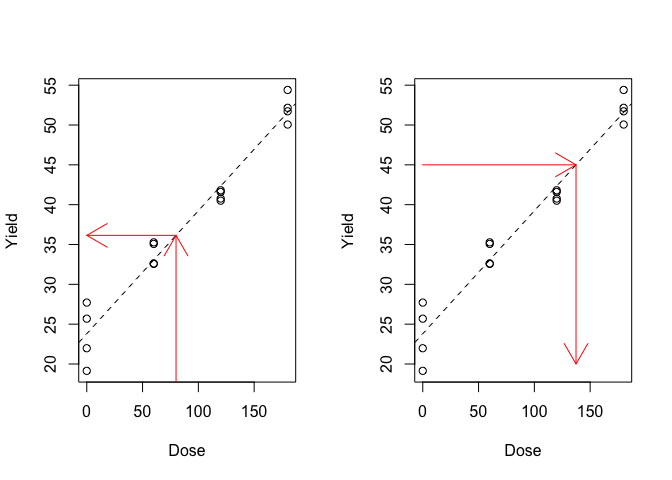
\includegraphics[width=0.9\linewidth]{_main_files/figure-latex/figName143-1} 

}

\caption{Esempio di previsioni: a destra, previsione della risposta per una data dose, a sinistra previsione della dose per ottenere una data risposta}\label{fig:figName143}
\end{figure}

Per entrambi i tipi di previsione ci si dovrebbe mantenere entro i livelli di dosi e risposte massimi e minimi inclusi ed osservati in prova, per evitare pericolose estrapolazioni (la risposta ha mostrato di essere lineare solo nell'intervallo osservato, ma non sappiamo cosa potrebbe capitare fuori da questo).

I parametri stimati possono essere facilmente utilizzati per fare previsioni dirette, come indicato nel box sottostante.

\begin{Shaded}
\begin{Highlighting}[]
\FloatTok{23.793750} \SpecialCharTok{+} \FloatTok{0.154417} \SpecialCharTok{*} \DecValTok{30}
\DocumentationTok{\#\# [1] 28.42626}
\FloatTok{23.793750} \SpecialCharTok{+} \FloatTok{0.154417} \SpecialCharTok{*} \DecValTok{80}
\DocumentationTok{\#\# [1] 36.14711}
\end{Highlighting}
\end{Shaded}

Anche queste stime, come tutte le altre, si riferiscono al campione in prova, mentre noi siamo interessati a fornire una previsione per l'intera popolazione da cui i nostri dati sono capionati. Per questo motivo, abbiamo la necessità di quantificare l'incertezza, attraverso un'opportuna stima dell'errore standard. In R, ciò è possibile utilizzando la funzione \texttt{predict()}, passando come argomento le dosi alle quali effettuare la previsione, organizzate in un data frame. Ad esempio, se si vuole prevedere la produzione a 30 e 80 kg N ha\textsuperscript{-1}, il codice è:

\begin{Shaded}
\begin{Highlighting}[]
\NormalTok{pred }\OtherTok{\textless{}{-}} \FunctionTok{predict}\NormalTok{(modelReg, }\AttributeTok{newdata=}\FunctionTok{data.frame}\NormalTok{(}\AttributeTok{Dose=}\FunctionTok{c}\NormalTok{(}\DecValTok{30}\NormalTok{, }\DecValTok{80}\NormalTok{)), }\AttributeTok{se=}\NormalTok{T)}
\NormalTok{pred}
\DocumentationTok{\#\# $fit}
\DocumentationTok{\#\#        1        2 }
\DocumentationTok{\#\# 28.42625 36.14708 }
\DocumentationTok{\#\# }
\DocumentationTok{\#\# $se.fit}
\DocumentationTok{\#\#         1         2 }
\DocumentationTok{\#\# 0.7519981 0.5666999 }
\DocumentationTok{\#\# }
\DocumentationTok{\#\# $df}
\DocumentationTok{\#\# [1] 14}
\DocumentationTok{\#\# }
\DocumentationTok{\#\# $residual.scale}
\DocumentationTok{\#\# [1] 2.242025}
\end{Highlighting}
\end{Shaded}

E'anche possibile effettuare la previsione inversa, cioè chiedere ai dati qual è la dose a cui corrisponde una produzione di 45 q/ha. In questo caso dobbiamo tener presente che l'equazione inversa è:

\[X = \frac{Y - b_0}{b_1}\]
e la previsione corrispondente è:

\begin{Shaded}
\begin{Highlighting}[]
\NormalTok{(}\DecValTok{45} \SpecialCharTok{{-}} \FloatTok{23.793750}\NormalTok{)}\SpecialCharTok{/}\FloatTok{0.154417}
\DocumentationTok{\#\# [1] 137.3311}
\end{Highlighting}
\end{Shaded}

Per determinare l'errore standard possiamo utilizzare la funzione \texttt{deltaMethod()}, nel package `car,' che ci calcola anche gli errori standard con il metodo della propagazione degli errori:

\begin{Shaded}
\begin{Highlighting}[]
\NormalTok{car}\SpecialCharTok{::}\FunctionTok{deltaMethod}\NormalTok{(modelReg, }\StringTok{"(45 {-} b0)/b1"}\NormalTok{, }
                 \AttributeTok{parameterNames=}\FunctionTok{c}\NormalTok{(}\StringTok{"b0"}\NormalTok{, }\StringTok{"b1"}\NormalTok{))}
\DocumentationTok{\#\#              Estimate       SE    2.5 \% 97.5 \%}
\DocumentationTok{\#\# (45 {-} b0)/b1 137.3314   4.4424 128.6244 146.04}
\end{Highlighting}
\end{Shaded}

Il procedimento sopra descritto è molto comune, per esempio nei laboratori chimici, dove viene utilizzato nella fase di calibrazione di uno strumento. Una volta che la retta di calibrazione è stata individuate, essa viene utilizzata per determinare le concentrazioni incognite di campioni per i quali sia stata misurata la risposta.

\begin{center}\rule{0.5\linewidth}{0.5pt}\end{center}

\hypertarget{altre-letture-9}{%
\section{Altre letture}\label{altre-letture-9}}

\begin{enumerate}
\def\labelenumi{\arabic{enumi}.}
\tightlist
\item
  Draper, N.R., Smith, H., 1981. Applied Regression Analysis, in: Applied Regression. John Wiley \& Sons, Inc., IDA, pp.~224--241.
\item
  Faraway, J.J., 2002. Practical regression and Anova using R. \url{http://cran.r-project.org/doc/contrib/Faraway-PRA.pdf}, R.
\end{enumerate}

\hypertarget{modelli-anova-a-due-vie}{%
\chapter{Modelli ANOVA a due vie}\label{modelli-anova-a-due-vie}}

Placeholder

\hypertarget{il-concetto-di-interazione}{%
\section{Il concetto di 'interazione'}\label{il-concetto-di-interazione}}

\hypertarget{tipi-di-interazione}{%
\section{Tipi di interazione}\label{tipi-di-interazione}}

\hypertarget{caso-studio-interazione-tra-lavorazioni-e-diserbo-chimico}{%
\section{Caso-studio: interazione tra lavorazioni e diserbo chimico}\label{caso-studio-interazione-tra-lavorazioni-e-diserbo-chimico}}

\hypertarget{definizione-del-modello-lineare-1}{%
\section{Definizione del modello lineare}\label{definizione-del-modello-lineare-1}}

\hypertarget{stima-dei-parametri-3}{%
\section{Stima dei parametri}\label{stima-dei-parametri-3}}

\hypertarget{verifica-delle-assunzioni-di-base}{%
\section{Verifica delle assunzioni di base}\label{verifica-delle-assunzioni-di-base}}

\hypertarget{scomposizione-delle-varianze}{%
\section{Scomposizione delle varianze}\label{scomposizione-delle-varianze}}

\hypertarget{medie-marginali-attese-1}{%
\section{Medie marginali attese}\label{medie-marginali-attese-1}}

\hypertarget{calcolo-degli-errori-standard-sem-e-sed}{%
\section{Calcolo degli errori standard (SEM e SED)}\label{calcolo-degli-errori-standard-sem-e-sed}}

\hypertarget{medie-marginali-attese-e-confronti-multipli-con-r}{%
\section{Medie marginali attese e confronti multipli con R}\label{medie-marginali-attese-e-confronti-multipli-con-r}}

\hypertarget{per-approfondire-un-po.}{%
\section{Per approfondire un po'\ldots.}\label{per-approfondire-un-po.}}

\hypertarget{anova-a-due-vie-scomposizione-manuale-della-varianza}{%
\subsection{Anova a due vie: scomposizione `manuale' della varianza}\label{anova-a-due-vie-scomposizione-manuale-della-varianza}}

\hypertarget{la-regressione-non-lineare}{%
\chapter{La regressione non-lineare}\label{la-regressione-non-lineare}}

Placeholder

\hypertarget{caso-studio-degradazione-di-un-erbicida-nel-terreno}{%
\section{Caso studio: degradazione di un erbicida nel terreno}\label{caso-studio-degradazione-di-un-erbicida-nel-terreno}}

\hypertarget{scelta-della-funzione}{%
\section{Scelta della funzione}\label{scelta-della-funzione}}

\hypertarget{stima-dei-parametri-4}{%
\section{Stima dei parametri}\label{stima-dei-parametri-4}}

\hypertarget{linearizzazione-della-funzione}{%
\subsection{Linearizzazione della funzione}\label{linearizzazione-della-funzione}}

\hypertarget{approssimazione-della-vera-funzione-tramite-una-polinomiale-in-x}{%
\subsection{Approssimazione della vera funzione tramite una polinomiale in X}\label{approssimazione-della-vera-funzione-tramite-una-polinomiale-in-x}}

\hypertarget{minimi-quadrati-non-lineari}{%
\subsection{Minimi quadrati non-lineari}\label{minimi-quadrati-non-lineari}}

\hypertarget{la-regressione-non-lineare-con-r}{%
\section{La regressione non-lineare con R}\label{la-regressione-non-lineare-con-r}}

\hypertarget{verifica-della-bontuxe0-del-modello}{%
\section{Verifica della bontà del modello}\label{verifica-della-bontuxe0-del-modello}}

\hypertarget{analisi-grafica-dei-residui-1}{%
\subsection{Analisi grafica dei residui}\label{analisi-grafica-dei-residui-1}}

\hypertarget{test-f-per-la-mancanza-di-adattamento-approssimato}{%
\subsection{Test F per la mancanza di adattamento (approssimato)}\label{test-f-per-la-mancanza-di-adattamento-approssimato}}

\hypertarget{errori-standard-dei-parametri-1}{%
\subsection{Errori standard dei parametri}\label{errori-standard-dei-parametri-1}}

\hypertarget{coefficienti-di-determinazione}{%
\subsection{Coefficienti di determinazione}\label{coefficienti-di-determinazione}}

\hypertarget{funzioni-lineari-e-nonlineari-dei-parametri}{%
\section{Funzioni lineari e nonlineari dei parametri}\label{funzioni-lineari-e-nonlineari-dei-parametri}}

\hypertarget{previsioni-1}{%
\section{Previsioni}\label{previsioni-1}}

\hypertarget{gestione-delle-situazioni-patologiche}{%
\section{Gestione delle situazioni `patologiche'}\label{gestione-delle-situazioni-patologiche}}

\hypertarget{trasformazione-del-modello}{%
\subsection{Trasformazione del modello}\label{trasformazione-del-modello}}

\hypertarget{trasformazione-dei-dati}{%
\subsection{Trasformazione dei dati}\label{trasformazione-dei-dati}}

\hypertarget{per-approfondire-un-po-1}{%
\section{Per approfondire un po'\ldots{}}\label{per-approfondire-un-po-1}}

\hypertarget{riparametrizzazione-delle-funzioni-non-lineari}{%
\subsection{Riparametrizzazione delle funzioni non-lineari}\label{riparametrizzazione-delle-funzioni-non-lineari}}

\hypertarget{altre-letture-10}{%
\subsection{Altre letture}\label{altre-letture-10}}

\hypertarget{esercizi}{%
\chapter{Esercizi}\label{esercizi}}

Placeholder

\hypertarget{capitoli-1-e-2}{%
\section{Capitoli 1 e 2}\label{capitoli-1-e-2}}

\hypertarget{esercizio-1}{%
\subsection{Esercizio 1}\label{esercizio-1}}

\hypertarget{capitolo-3}{%
\section{Capitolo 3}\label{capitolo-3}}

\hypertarget{esercizio-1-1}{%
\subsection{Esercizio 1}\label{esercizio-1-1}}

\hypertarget{esercizio-2}{%
\subsection{Esercizio 2}\label{esercizio-2}}

\hypertarget{esercizio-3}{%
\subsection{Esercizio 3}\label{esercizio-3}}

\hypertarget{capitolo-4}{%
\section{Capitolo 4}\label{capitolo-4}}

\hypertarget{esercizio-1-2}{%
\subsection{Esercizio 1}\label{esercizio-1-2}}

\hypertarget{esercizio-2-1}{%
\subsection{Esercizio 2}\label{esercizio-2-1}}

\hypertarget{esercizio-3-1}{%
\subsection{Esercizio 3}\label{esercizio-3-1}}

\hypertarget{esercizio-4}{%
\subsection{Esercizio 4}\label{esercizio-4}}

\hypertarget{esercizio-5}{%
\subsection{Esercizio 5}\label{esercizio-5}}

\hypertarget{esercizio-6}{%
\subsection{Esercizio 6}\label{esercizio-6}}

\hypertarget{esercizio-7}{%
\subsection{Esercizio 7}\label{esercizio-7}}

\hypertarget{esercizio-8}{%
\subsection{Esercizio 8}\label{esercizio-8}}

\hypertarget{capitolo-5}{%
\section{Capitolo 5}\label{capitolo-5}}

\hypertarget{esercizio-1-3}{%
\subsection{Esercizio 1}\label{esercizio-1-3}}

\hypertarget{esercizio-2-2}{%
\subsection{Esercizio 2}\label{esercizio-2-2}}

\hypertarget{esercizio-3-2}{%
\subsection{Esercizio 3}\label{esercizio-3-2}}

\hypertarget{esercizio-4-1}{%
\subsection{Esercizio 4}\label{esercizio-4-1}}

\hypertarget{esercizio-5-1}{%
\subsection{Esercizio 5}\label{esercizio-5-1}}

\hypertarget{capitolo-6}{%
\section{Capitolo 6}\label{capitolo-6}}

\hypertarget{esercizio-1-4}{%
\subsection{Esercizio 1}\label{esercizio-1-4}}

\hypertarget{esercizio-2-3}{%
\subsection{Esercizio 2}\label{esercizio-2-3}}

\hypertarget{esercizio-3-3}{%
\subsection{Esercizio 3}\label{esercizio-3-3}}

\hypertarget{esercizio-4-2}{%
\subsection{Esercizio 4}\label{esercizio-4-2}}

\hypertarget{esercizio-5-2}{%
\subsection{Esercizio 5}\label{esercizio-5-2}}

\hypertarget{esercizio-6-1}{%
\subsection{Esercizio 6}\label{esercizio-6-1}}

\hypertarget{esercizio-7-1}{%
\subsection{Esercizio 7}\label{esercizio-7-1}}

\hypertarget{esercizio-8-1}{%
\subsection{Esercizio 8}\label{esercizio-8-1}}

\hypertarget{esercizio-9}{%
\subsection{Esercizio 9}\label{esercizio-9}}

\hypertarget{esercizio-10}{%
\subsection{Esercizio 10}\label{esercizio-10}}

\hypertarget{capitoli-da-7-a-9}{%
\section{Capitoli da 7 a 9}\label{capitoli-da-7-a-9}}

\hypertarget{esercizio-1-5}{%
\subsection{Esercizio 1}\label{esercizio-1-5}}

\hypertarget{esercizio-2-4}{%
\subsection{Esercizio 2}\label{esercizio-2-4}}

\hypertarget{esercizio-3-4}{%
\subsection{Esercizio 3}\label{esercizio-3-4}}

\hypertarget{esercizio-4-3}{%
\subsection{Esercizio 4}\label{esercizio-4-3}}

\hypertarget{capitolo-10}{%
\section{Capitolo 10}\label{capitolo-10}}

\hypertarget{esercizio-1-6}{%
\subsection{Esercizio 1}\label{esercizio-1-6}}

\hypertarget{esercizio-2-5}{%
\subsection{Esercizio 2}\label{esercizio-2-5}}

\hypertarget{esercizio-3-5}{%
\subsection{Esercizio 3}\label{esercizio-3-5}}

\hypertarget{capitoli-11-e-12}{%
\section{Capitoli 11 e 12}\label{capitoli-11-e-12}}

\hypertarget{esercizio-1-7}{%
\subsection{Esercizio 1}\label{esercizio-1-7}}

\hypertarget{esercizio-2-6}{%
\subsection{Esercizio 2}\label{esercizio-2-6}}

\hypertarget{esercizio-3-6}{%
\subsection{Esercizio 3}\label{esercizio-3-6}}

\hypertarget{esercizio-4-4}{%
\subsection{Esercizio 4}\label{esercizio-4-4}}

\hypertarget{esercizio-5-3}{%
\subsection{Esercizio 5}\label{esercizio-5-3}}

\hypertarget{esercizio-6-2}{%
\subsection{Esercizio 6}\label{esercizio-6-2}}

\hypertarget{capitolo-13}{%
\section{Capitolo 13}\label{capitolo-13}}

\hypertarget{esercizio-1-8}{%
\subsection{Esercizio 1}\label{esercizio-1-8}}

\hypertarget{esercizio-2-7}{%
\subsection{Esercizio 2}\label{esercizio-2-7}}

\hypertarget{capitolo-14}{%
\section{Capitolo 14}\label{capitolo-14}}

\hypertarget{esercizio-1-9}{%
\subsection{Esercizio 1}\label{esercizio-1-9}}

\hypertarget{esercizio-2-8}{%
\subsection{Esercizio 2}\label{esercizio-2-8}}

\hypertarget{esercizio-3-7}{%
\subsection{Esercizio 3}\label{esercizio-3-7}}

\hypertarget{esercizio-4-5}{%
\subsection{Esercizio 4}\label{esercizio-4-5}}

\hypertarget{esercizio-5-4}{%
\subsection{Esercizio 5}\label{esercizio-5-4}}

\hypertarget{esercizio-6-3}{%
\subsection{Esercizio 6}\label{esercizio-6-3}}

\hypertarget{esercizio-7-2}{%
\subsection{Esercizio 7}\label{esercizio-7-2}}

\hypertarget{appendice-1-breve-introduzione-ad-r}{%
\chapter{Appendice 1: breve introduzione ad R}\label{appendice-1-breve-introduzione-ad-r}}

Placeholder

\hypertarget{cosa-uxe8-r}{%
\section*{Cosa è R?}\label{cosa-uxe8-r}}
\addcontentsline{toc}{section}{Cosa è R?}

\hypertarget{oggetti-e-assegnazioni}{%
\section*{Oggetti e assegnazioni}\label{oggetti-e-assegnazioni}}
\addcontentsline{toc}{section}{Oggetti e assegnazioni}

\hypertarget{costanti-e-vettori}{%
\subsection*{Costanti e vettori}\label{costanti-e-vettori}}
\addcontentsline{toc}{subsection}{Costanti e vettori}

\hypertarget{matrici}{%
\subsection*{Matrici}\label{matrici}}
\addcontentsline{toc}{subsection}{Matrici}

\hypertarget{dataframe}{%
\subsection*{Dataframe}\label{dataframe}}
\addcontentsline{toc}{subsection}{Dataframe}

\hypertarget{quale-oggetto-sto-utilizzando}{%
\subsection*{Quale oggetto sto utilizzando?}\label{quale-oggetto-sto-utilizzando}}
\addcontentsline{toc}{subsection}{Quale oggetto sto utilizzando?}

\hypertarget{operazioni-ed-operatori}{%
\section*{Operazioni ed operatori}\label{operazioni-ed-operatori}}
\addcontentsline{toc}{section}{Operazioni ed operatori}

\hypertarget{funzioni-ed-argomenti}{%
\section*{Funzioni ed argomenti}\label{funzioni-ed-argomenti}}
\addcontentsline{toc}{section}{Funzioni ed argomenti}

\hypertarget{consigli-per-limmissione-di-dati-sperimentali}{%
\section*{Consigli per l'immissione di dati sperimentali}\label{consigli-per-limmissione-di-dati-sperimentali}}
\addcontentsline{toc}{section}{Consigli per l'immissione di dati sperimentali}

\hypertarget{immissione-di-numeri-progressivi}{%
\subsection*{Immissione di numeri progressivi}\label{immissione-di-numeri-progressivi}}
\addcontentsline{toc}{subsection}{Immissione di numeri progressivi}

\hypertarget{immissione-dei-codici-delle-tesi-e-dei-blocchi}{%
\subsection*{Immissione dei codici delle tesi e dei blocchi}\label{immissione-dei-codici-delle-tesi-e-dei-blocchi}}
\addcontentsline{toc}{subsection}{Immissione dei codici delle tesi e dei blocchi}

\hypertarget{immissione-dei-valori-e-creazione-del-datframe}{%
\subsection*{Immissione dei valori e creazione del datframe}\label{immissione-dei-valori-e-creazione-del-datframe}}
\addcontentsline{toc}{subsection}{Immissione dei valori e creazione del datframe}

\hypertarget{leggere-e-salvare-dati-esterni}{%
\subsection*{Leggere e salvare dati esterni}\label{leggere-e-salvare-dati-esterni}}
\addcontentsline{toc}{subsection}{Leggere e salvare dati esterni}

\hypertarget{alcune-operazioni-comuni-sul-dataset}{%
\section*{Alcune operazioni comuni sul dataset}\label{alcune-operazioni-comuni-sul-dataset}}
\addcontentsline{toc}{section}{Alcune operazioni comuni sul dataset}

\hypertarget{selezionare-un-subset-di-dati}{%
\subsection*{Selezionare un subset di dati}\label{selezionare-un-subset-di-dati}}
\addcontentsline{toc}{subsection}{Selezionare un subset di dati}

\hypertarget{ordinare-un-vettore-o-un-dataframe}{%
\subsection*{Ordinare un vettore o un dataframe}\label{ordinare-un-vettore-o-un-dataframe}}
\addcontentsline{toc}{subsection}{Ordinare un vettore o un dataframe}

\hypertarget{workspace}{%
\section*{Workspace}\label{workspace}}
\addcontentsline{toc}{section}{Workspace}

\hypertarget{script-o-programmi}{%
\section*{Script o programmi}\label{script-o-programmi}}
\addcontentsline{toc}{section}{Script o programmi}

\hypertarget{interrogazione-di-oggetti}{%
\section*{Interrogazione di oggetti}\label{interrogazione-di-oggetti}}
\addcontentsline{toc}{section}{Interrogazione di oggetti}

\hypertarget{altre-funzioni-matriciali}{%
\section*{Altre funzioni matriciali}\label{altre-funzioni-matriciali}}
\addcontentsline{toc}{section}{Altre funzioni matriciali}

\hypertarget{cenni-sulle-funzionalituxe0-grafiche-in-r}{%
\section*{Cenni sulle funzionalità grafiche in R}\label{cenni-sulle-funzionalituxe0-grafiche-in-r}}
\addcontentsline{toc}{section}{Cenni sulle funzionalità grafiche in R}

\hypertarget{altre-letture-11}{%
\section*{Altre letture}\label{altre-letture-11}}
\addcontentsline{toc}{section}{Altre letture}


\end{document}
